\chapter{Azure}
% \capepigrafe[0.5\textwidth]{``Uma frase bem legal sobre o legado deixado''}{Autor da frase bem legal}


\section{Introdução}
A Azure é uma plataforma de computação em nuvem, agindo como provedor \textit{SaaS, PaaS} e \textit{Iaas}. Tem como proprietária a empresa americana \textit{Microsoft}, e disponibiliza serviços como \textit{builds}, testes, \textit{deploys} e gerenciamento de aplicações que estão hospedadas em \textit{data centers} administrados pela própria empresa.

Atualmente possui mais de 600 ferramentas para os mais diversos usos na área da computação, como serviços de armazenamento, soluções para desenvolvimento \textit{Mobile}, administração de dados, messageria, CDN e etc. Além disso, seus \textit{data centers} que constituem 36 regiões ao redor do globo, provendo estabilidade e escalabilidade sem problemas de latência.

\begin{figure}[h!]
  \centering
  \includegraphics[scale=0.38]{imagens/azure-regions.eps}
  \caption{Regiões disponibilizadas pela Azure}
\end{figure}

\section{Vantagens e diferenciais}
O primeiro atributo positivo a considerar em relação aos serviços de nuvem da Azure é a confiabilidade da infraestura do provedor. Seu Contrato de Nível de Serviço (em inglês, \textit{SLA}) estima uma porcentagem de disponibilibade de 99,95\%, o que equivale a pouco mais de quatro horas anuais de tempo de \textit{downtime}. Essa é uma conquista que até mesmo uma solução \textit{on premises} simplesmente não consegue atingir de forma consistente. No entanto, hospedar um aplicativo ou armazenar dados na nuvem geralmente está associado a uma alta disponibilidade - certamente um dos maiores apelos de \textit{cloud computing}. Porém a alta disponibilidade dos Serviços de Nuvem do Azure da \textit{Microsoft} continua a impressionar, inspirando muitas vezes \textit{CIOs} a migrar pelo menos uma parte de suas soluções mais pesadas de dados \textit{on-line}.

Além disso, uma das maiores preocupações das empresas ao migrar para a nuvem é a segurança. A Azure segue o modelo de segurança padrão, que consiste em ``detectar, avaliar, diagnosticar, estabilizar e fechar''. Esse modelo, alinhado com outras políticas rígidas de segurança, rendeu à plataforma uma séria de certificações de \textit{compliance}, a estabelecendo como líder em segurança de \textit{IaaS}. Fornece proteção em vários níveis e serviços simples e fáceis de usar.


\begin{figure}[h!]
  \centering
  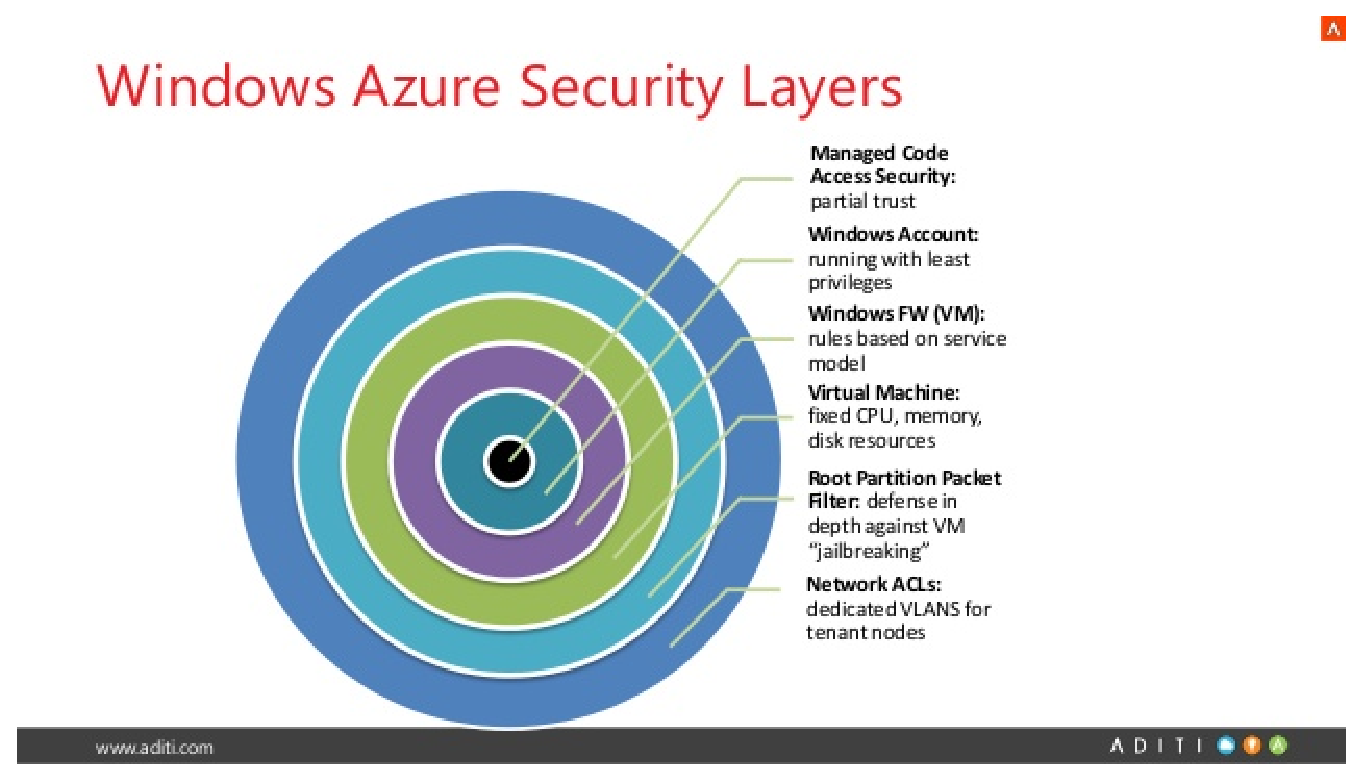
\includegraphics[scale=0.75]{imagens/azure-security.eps}
  \caption{Camadas de Segurança da Azure}
\end{figure}

\newpage

Finalmente, os serviços de nuvem da Azure também oferecem a escalabilidade necessária para o crescimento de qualquer solução, fornecendo maior poder computacional conforme necessário. Seja uma pequena empresa, ou uma empresa com a necessidade de um grande \textit{data warehouse}, os serviços de nuvem do Azure têm armazenamento e capacidade computacional para lidar com praticamente qualquer tipo de demanda.


 
\section{Desvantagens}

Ao contrário das plataformas \textit{SaaS}, nas quais o usuário final está consumindo informações (por exemplo, o \textit{Office 365}), a Azure migra o poder computacional de dentro de sua empresa \textit{(datacenter)} ou escritório para a nuvem. Como ocorre com a maioria dos provedores de serviços em nuvem, o Azure precisa ser gerenciado e mantido cuidadosamente, o que inclui aplicação de \textit{patches} e o monitoramento dos servidores.

Ao contrário dos servidores locais, o Azure exige experiência para garantir que todas as partes móveis trabalhem juntas de forma eficiente. Um erro comum dos administradores de negócios que não estão totalmente envolvidos em quão bem (ou mal) seus servidores de nuvem estão operando é o de fazer o chamado \textit{over-provisioning} dos serviços em nuvem. Embora seja um erro corriqueiro, essa falta de conhecimento dos administradores pode custar às empresas milhares de dólares por ano.


\section{Conclusão}
No geral, a Azure é uma excelente plataforma de  \textit{cloud computing}, ficando atrás de seus concorrentes apenas em alguns poucos pontos. Possui serviços robustos e bem consolidados, bastante segurança, e boa disponibilidade e escalabilidade. Além disso, torna-se quase que uma escolha obrigatória para empresas que já utilizam ou tem familiaridade com ambientes \textit{Microsoft}, devido às inúmeras facilidades extras fornecidas (integrações e possíveis cortes de gastos com licenças).  
